As this analysis selects only high-\pt-ID muons, a significant fraction of muons are in a momentum space where reconstruction relies less on the inner tracker and more on the muon system. While tracker-derived Rochester corrections adequately scale lower muon momenta, these corrections---and corresponding uncertainty estimates---do not cover muons at high \pt. To overcome this limitation and estimate a MES uncertainty at muon \pt beyond the \SI{200}{\GeV} threshold of the Rochester scale corrections, we use the Generalized Endpoint (GE) method to estimate an uncertainty of scale bias for muons with $\pt > \SI{200}{\GeV}$. This partitioning of the MES uncertainty estimation follows the recommendations set by the Muon POG for high-\pt ID muons provided on the Twiki pages in Refs. \cite{MuonTwiki2016,MuonTwiki2018}. The GE method uses statistical replicas of scale bias maps binned in $\phi$ and \pseudorap, where each element of a copy $\kappa_{b,\,\text{copy}}$ is drawn from a gaussian distribution whose mean is the measured bias $\kappa_b$ and standard deviation is the measurement uncertainty $\sigma$. For each copy, muon \pt is translated by:
\begin{equation}
    \frac{q}{\pt} \rightarrow \frac{q}{\pt} + \kappa_{b,\,\text{copy}},
\end{equation}
giving:
\begin{equation}
    \pt \rightarrow \frac{\pt}{1 + q\pt\kappa_{b,\,\text{copy}}},
\end{equation}
where $q$ is the electric charge of the muon. The momentum translations are propagated to final results (defined below) for each copy and averaged, and the uncertainty estimated from the relative difference in events between nominal and average distributions (for the contribution from data-normalized \ZJETS and \ttbar backgrounds we use the relative difference in efficiency rather than the relative difference in the number of events). Premade copies of scale biases and momentum translations are available through the GEScaleSyst package on GitLab~\cite{GEScaleSyst}. Figure~\ref{figapp:gesysmuonptBkg} shows the nominal muon \pt compared to the corresponding statistical replicas and averaged distributions in background MC at preselection, while Figs.~\ref{figapp:gesysBDTscoresSig1} and~\ref{figapp:gesysBDTscoresSig2} show the nominal BDT scores of select masses compared to the corresponding statistical replicas and averaged distributions in signal MC at preselection. 

The selection criteria used to estimate the GE scale uncertainty was studied at five working points, corresponding to different cuts on the BDT scores. Along with preselection, $\Muu > \SI{250}{\GeV}$ and $\Muujj > \MLQ$ requirements were additionally applied to data at all working points. Each working point was defined by the following cut:
\begin{itemize}
    \item Enhanced: BDT score $\geq 0.0$
    \item Loose: BDT score $> 0.1$
    \item Medium: BDT score $> 0.5$
    \item Tight: BDT score $> 0.9$
    \item Optimized: BDT score $>$ optimized cut (see: Table~\ref{tab:cutlog})
\end{itemize}
The uncertainty estimated with the GE method at each working point and leptoquark mass point in background and signal MC are listed in Tables~\ref{tab:gesystbkg} and~\ref{tab:gesystsig}, respectively. This analysis uses the enhanced working point to estimate the GE scale uncertainty, as it is loose enough (with no cut on the BDT score) to retain sufficient statics, while the cut on $\Muujj > \MLQ$ ensures events are characterized by the same kinematics as the signal region.

\begin{figure}[H]
    \centering
    {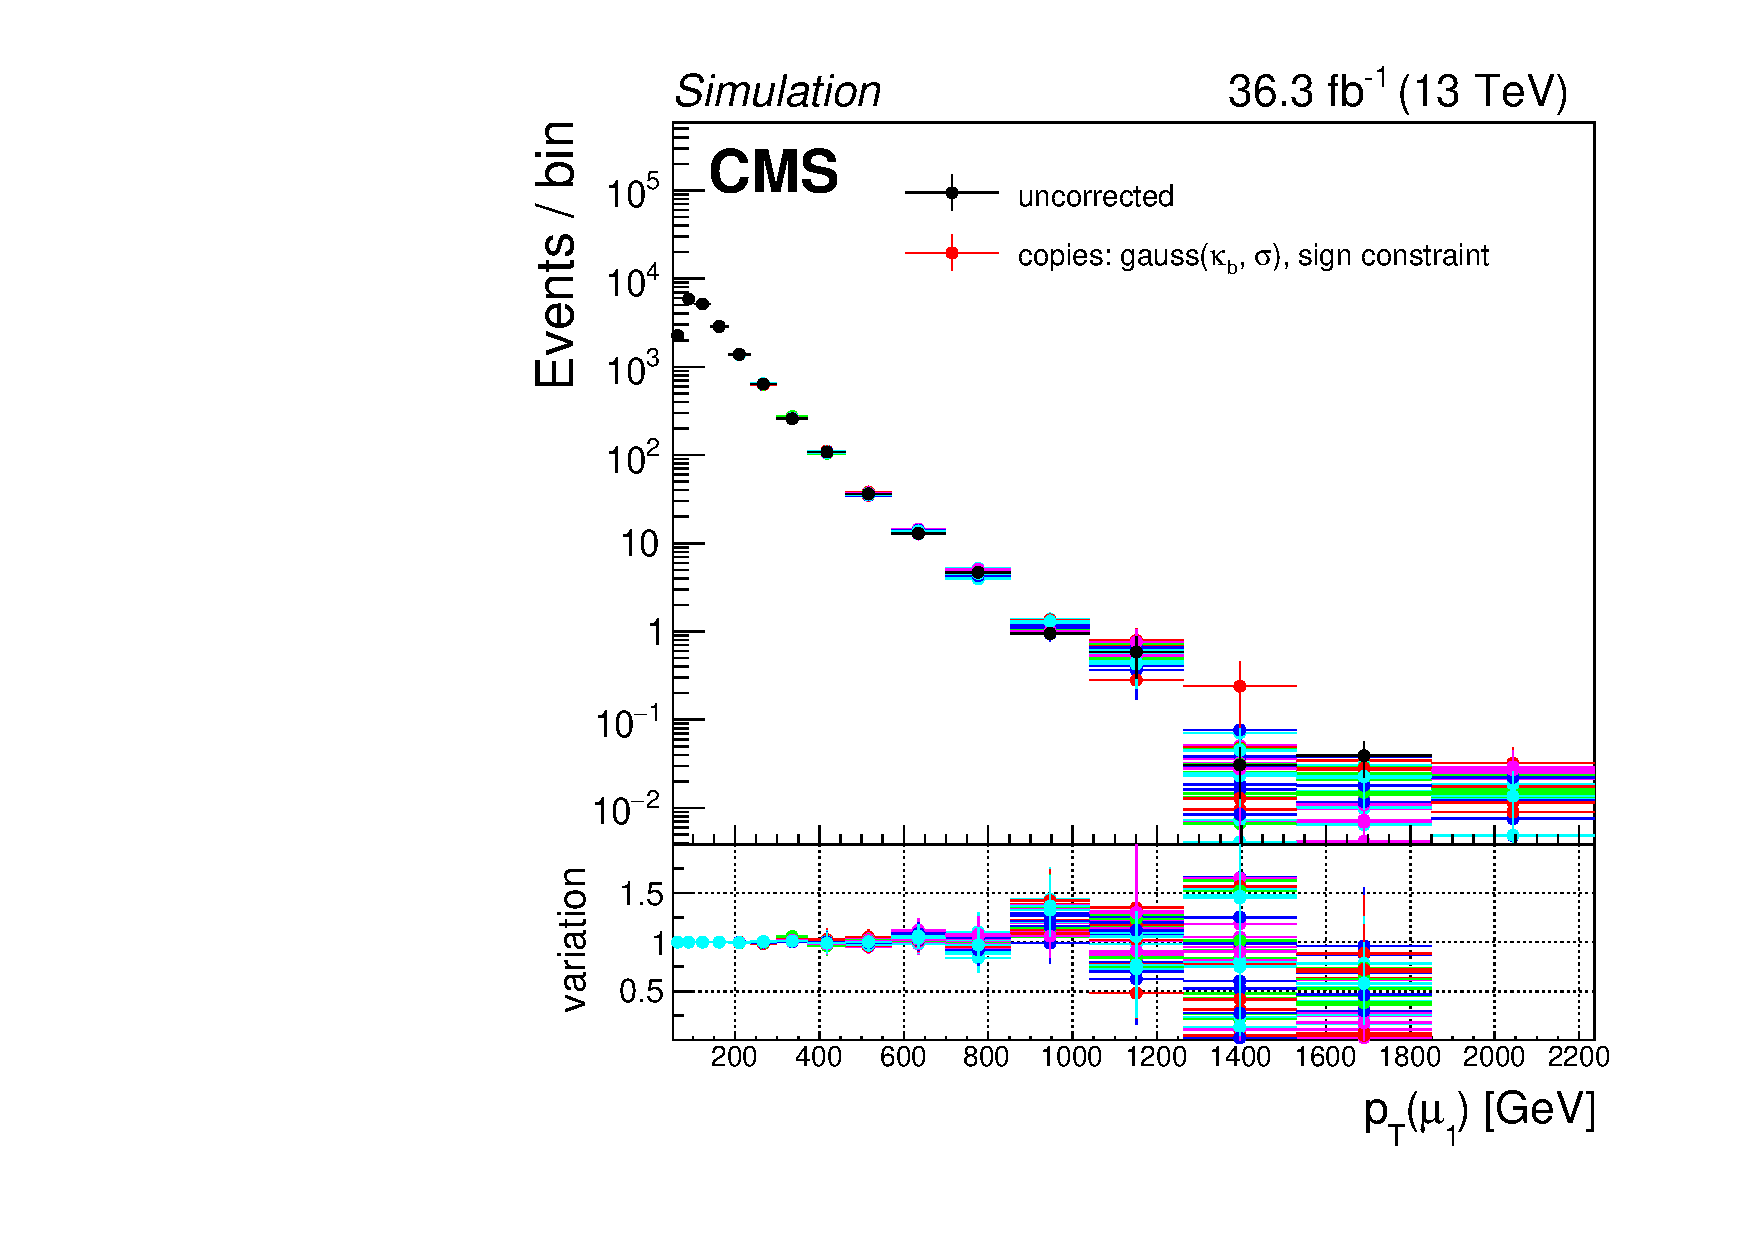
\includegraphics[width=.49\textwidth]{Images/Analysis/GEScaleSystStudy/StudyPlots_2016/Background/Copies/preSel/GEScaleSystStudyPlot_2016_Background_Copies_preSel_Pt_muon1.pdf}}
    {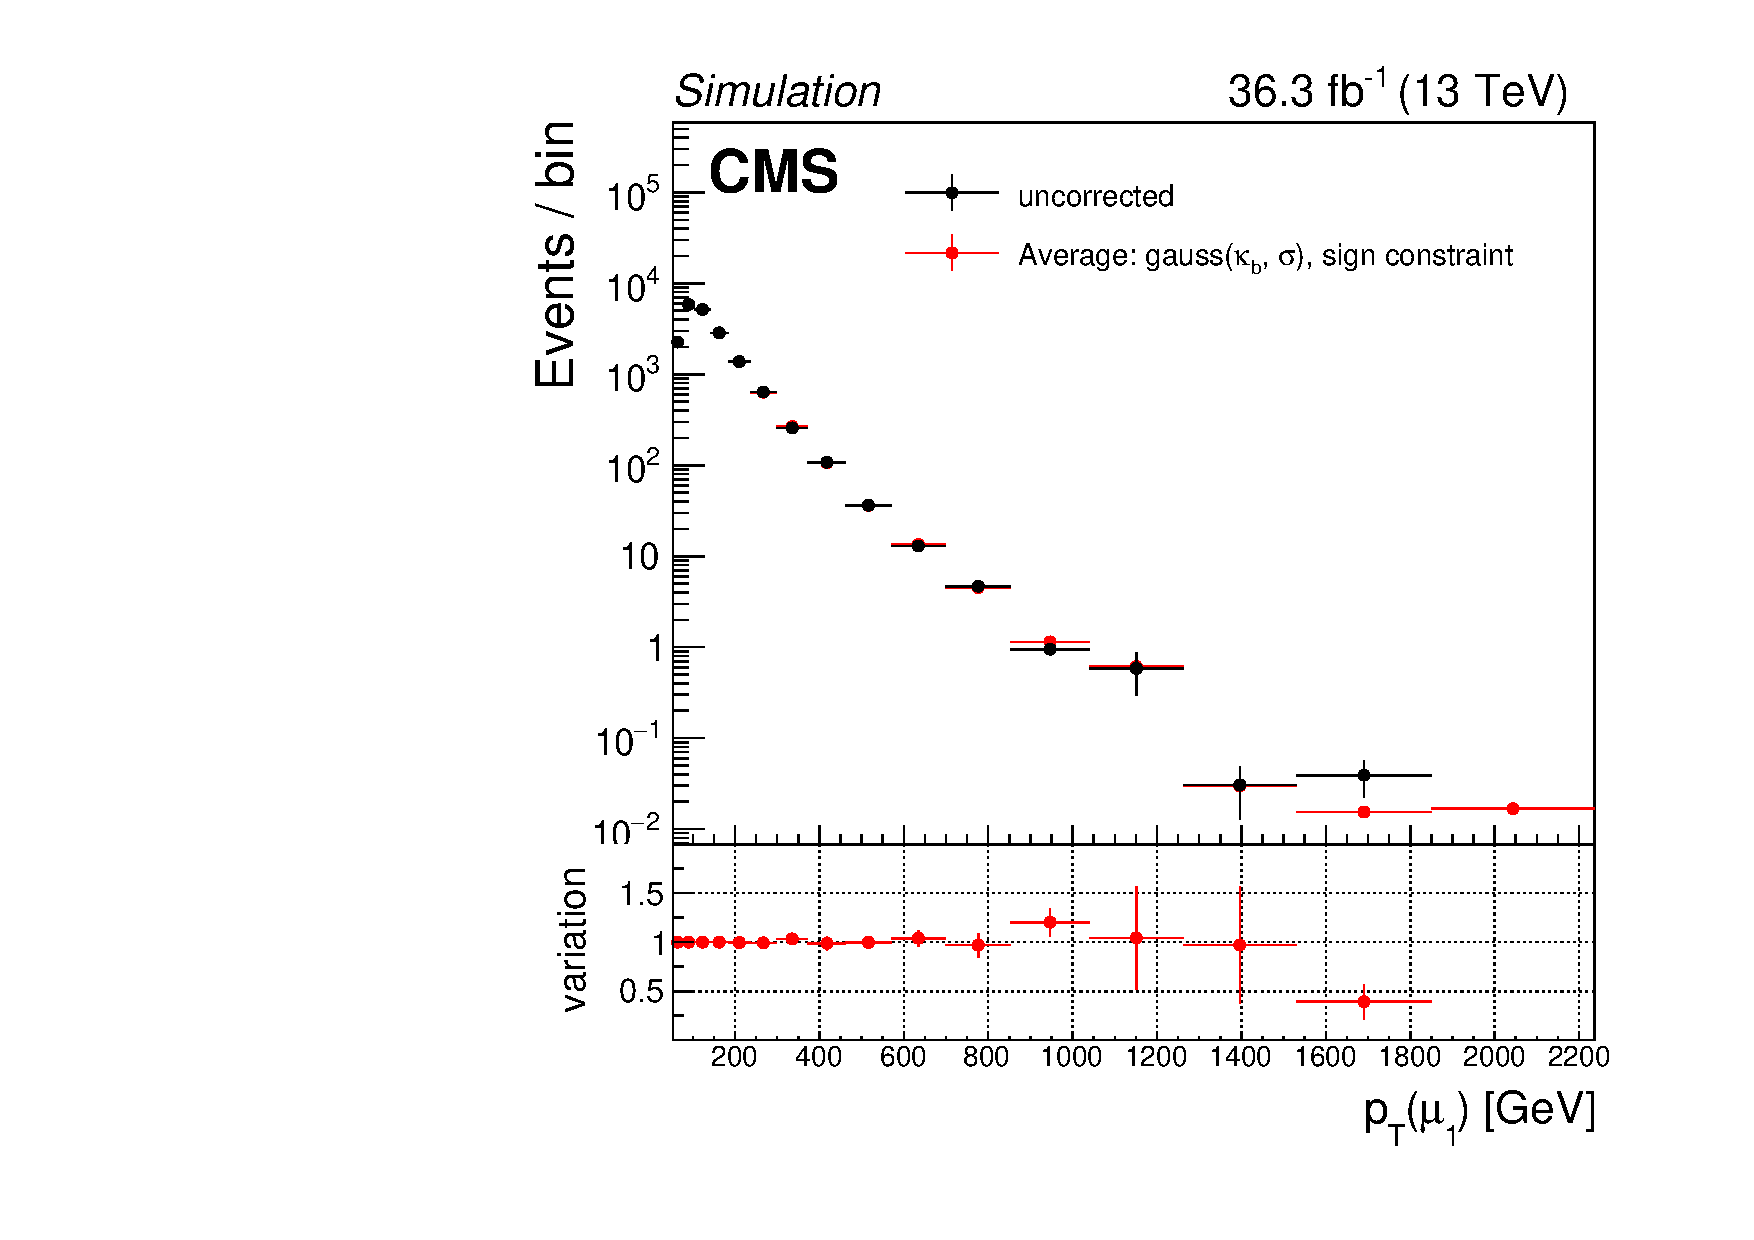
\includegraphics[width=.49\textwidth]{Images/Analysis/GEScaleSystStudy/StudyPlots_2016/Background/Averages/preSel/GEScaleSystStudyPlot_2016_Background_Average_preSel_Pt_muon1.pdf}}
    {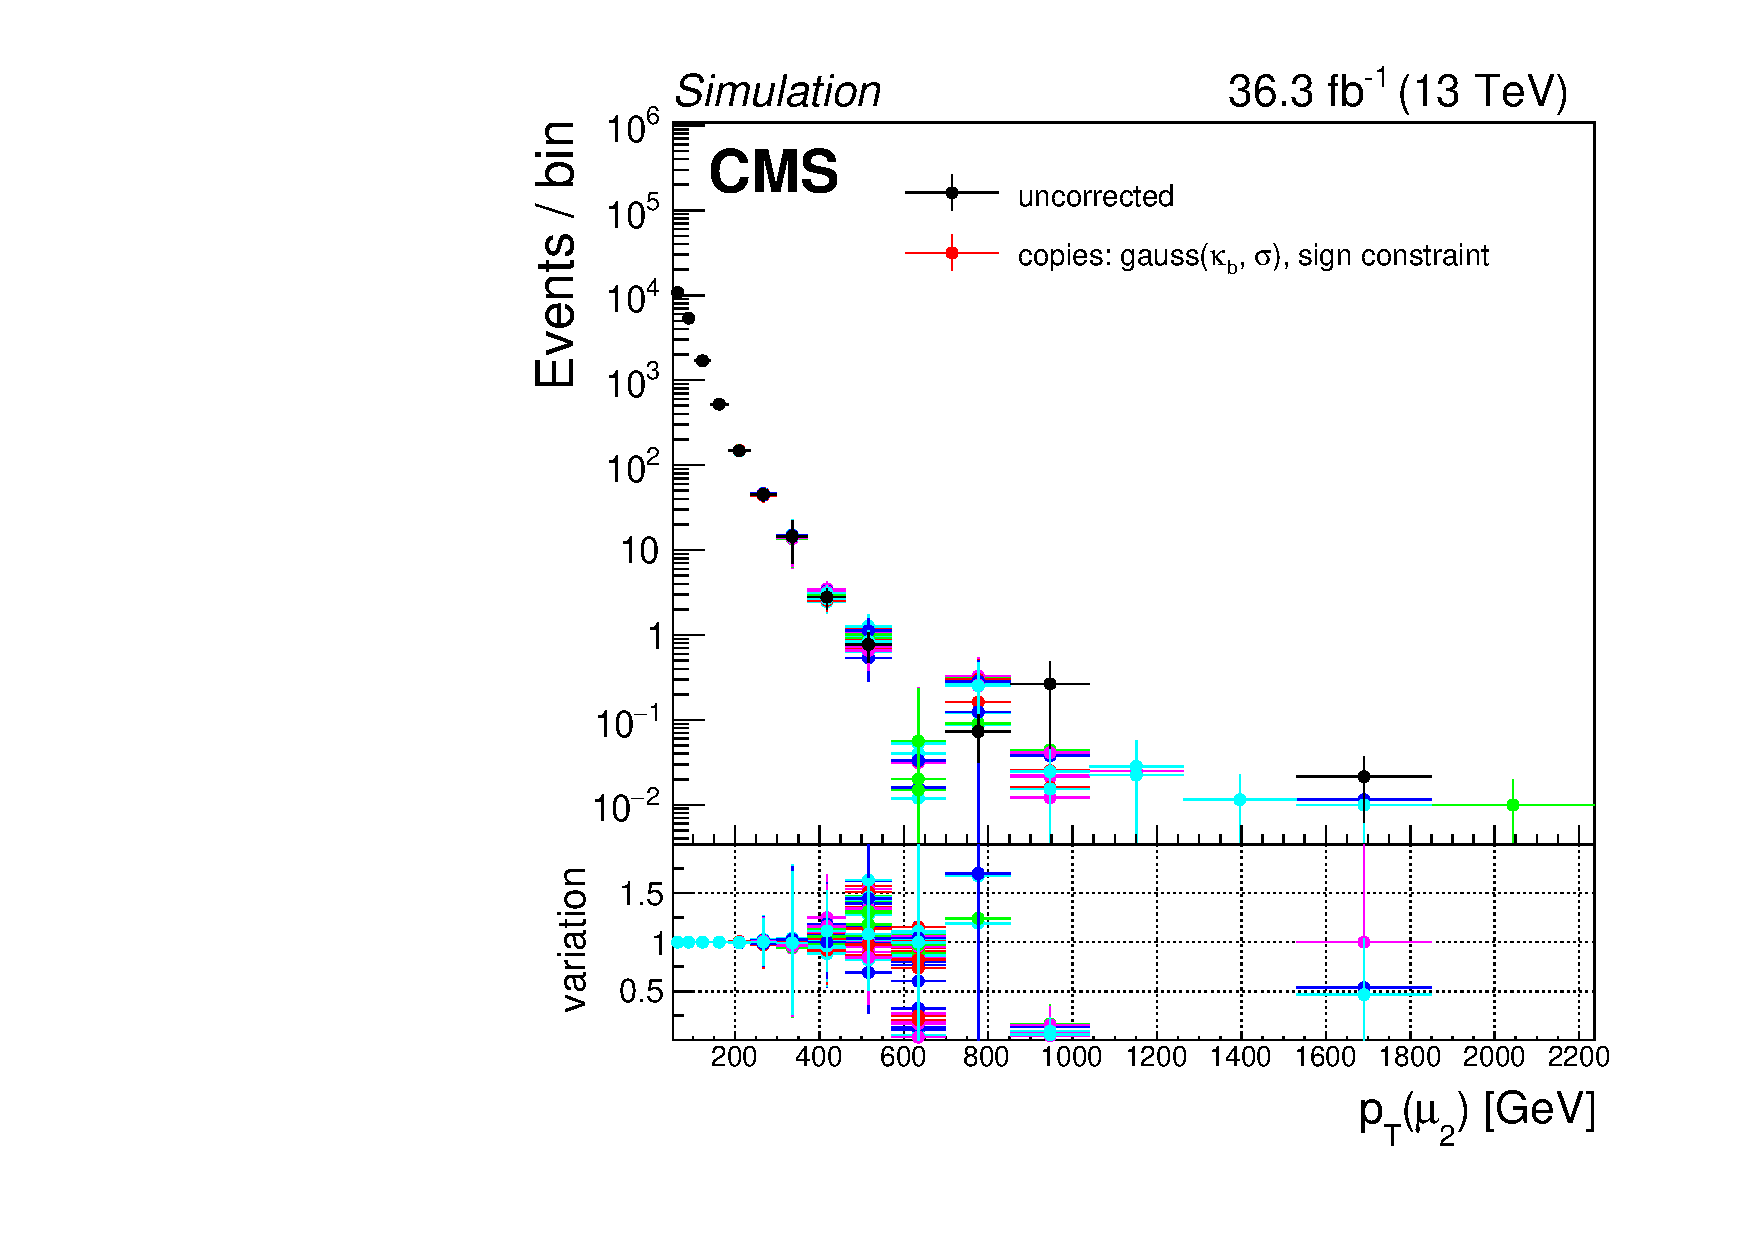
\includegraphics[width=.49\textwidth]{Images/Analysis/GEScaleSystStudy/StudyPlots_2016/Background/Copies/preSel/GEScaleSystStudyPlot_2016_Background_Copies_preSel_Pt_muon2.pdf}}
    {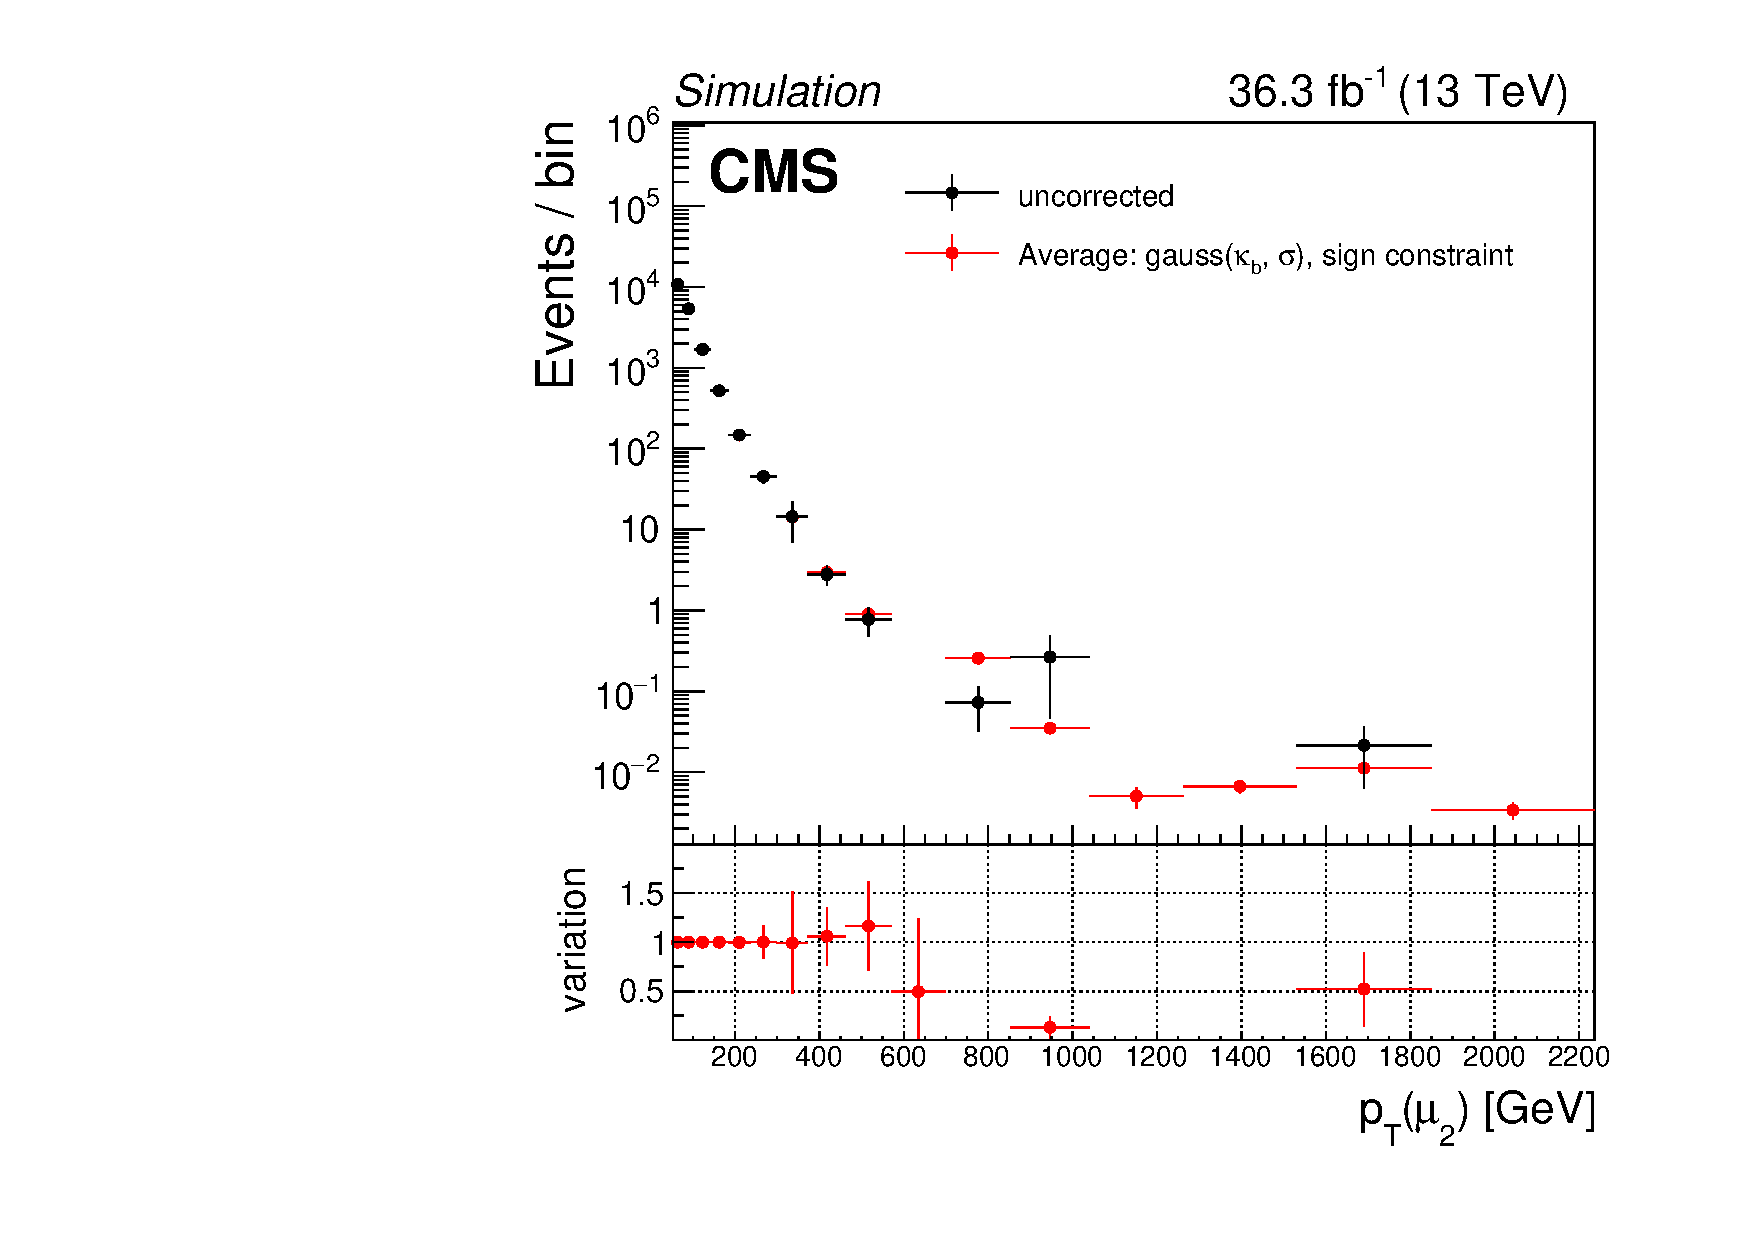
\includegraphics[width=.49\textwidth]{Images/Analysis/GEScaleSystStudy/StudyPlots_2016/Background/Averages/preSel/GEScaleSystStudyPlot_2016_Background_Average_preSel_Pt_muon2.pdf}}
    \caption{Left: A comparison between the nominal and statistical replicas of muon 1 \pt (top) and muon 2 \pt (bottom). Right: A comparison between the nominal and average over the statistical replicas of muon 1 \pt (top) and muon 2 \pt (bottom). Distributions show 2016 background MC at preselection.}
    \label{figapp:gesysmuonptBkg}
\end{figure}

\begin{figure}[H]
    \centering
    {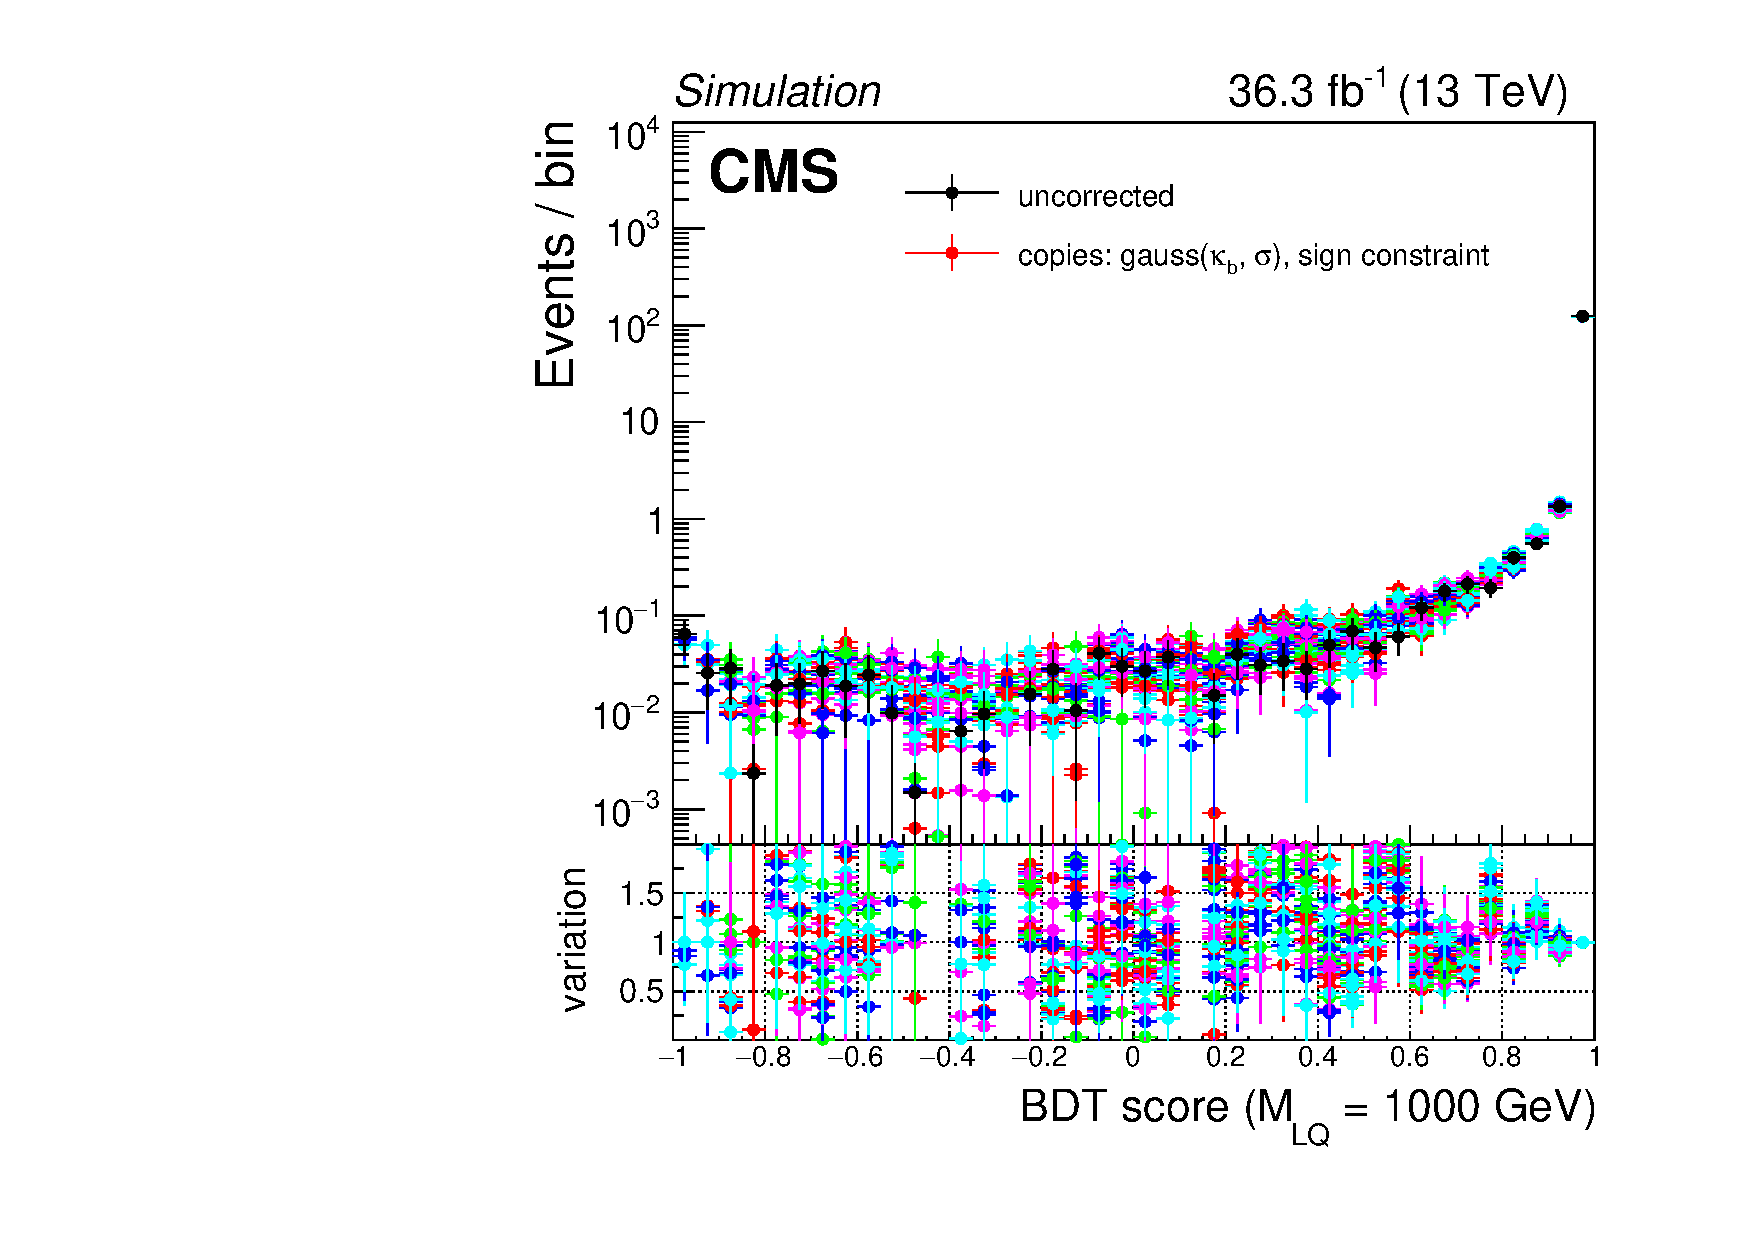
\includegraphics[width=.49\textwidth]{Images/Analysis/GEScaleSystStudy/StudyPlots_2016/SignalM1000/Copies/preSel/GEScaleSystStudyPlot_2016_SignalM1000_Copies_preSel_LQToBMu_pair_uubj_BDT_discrim_M1000.pdf}}
    {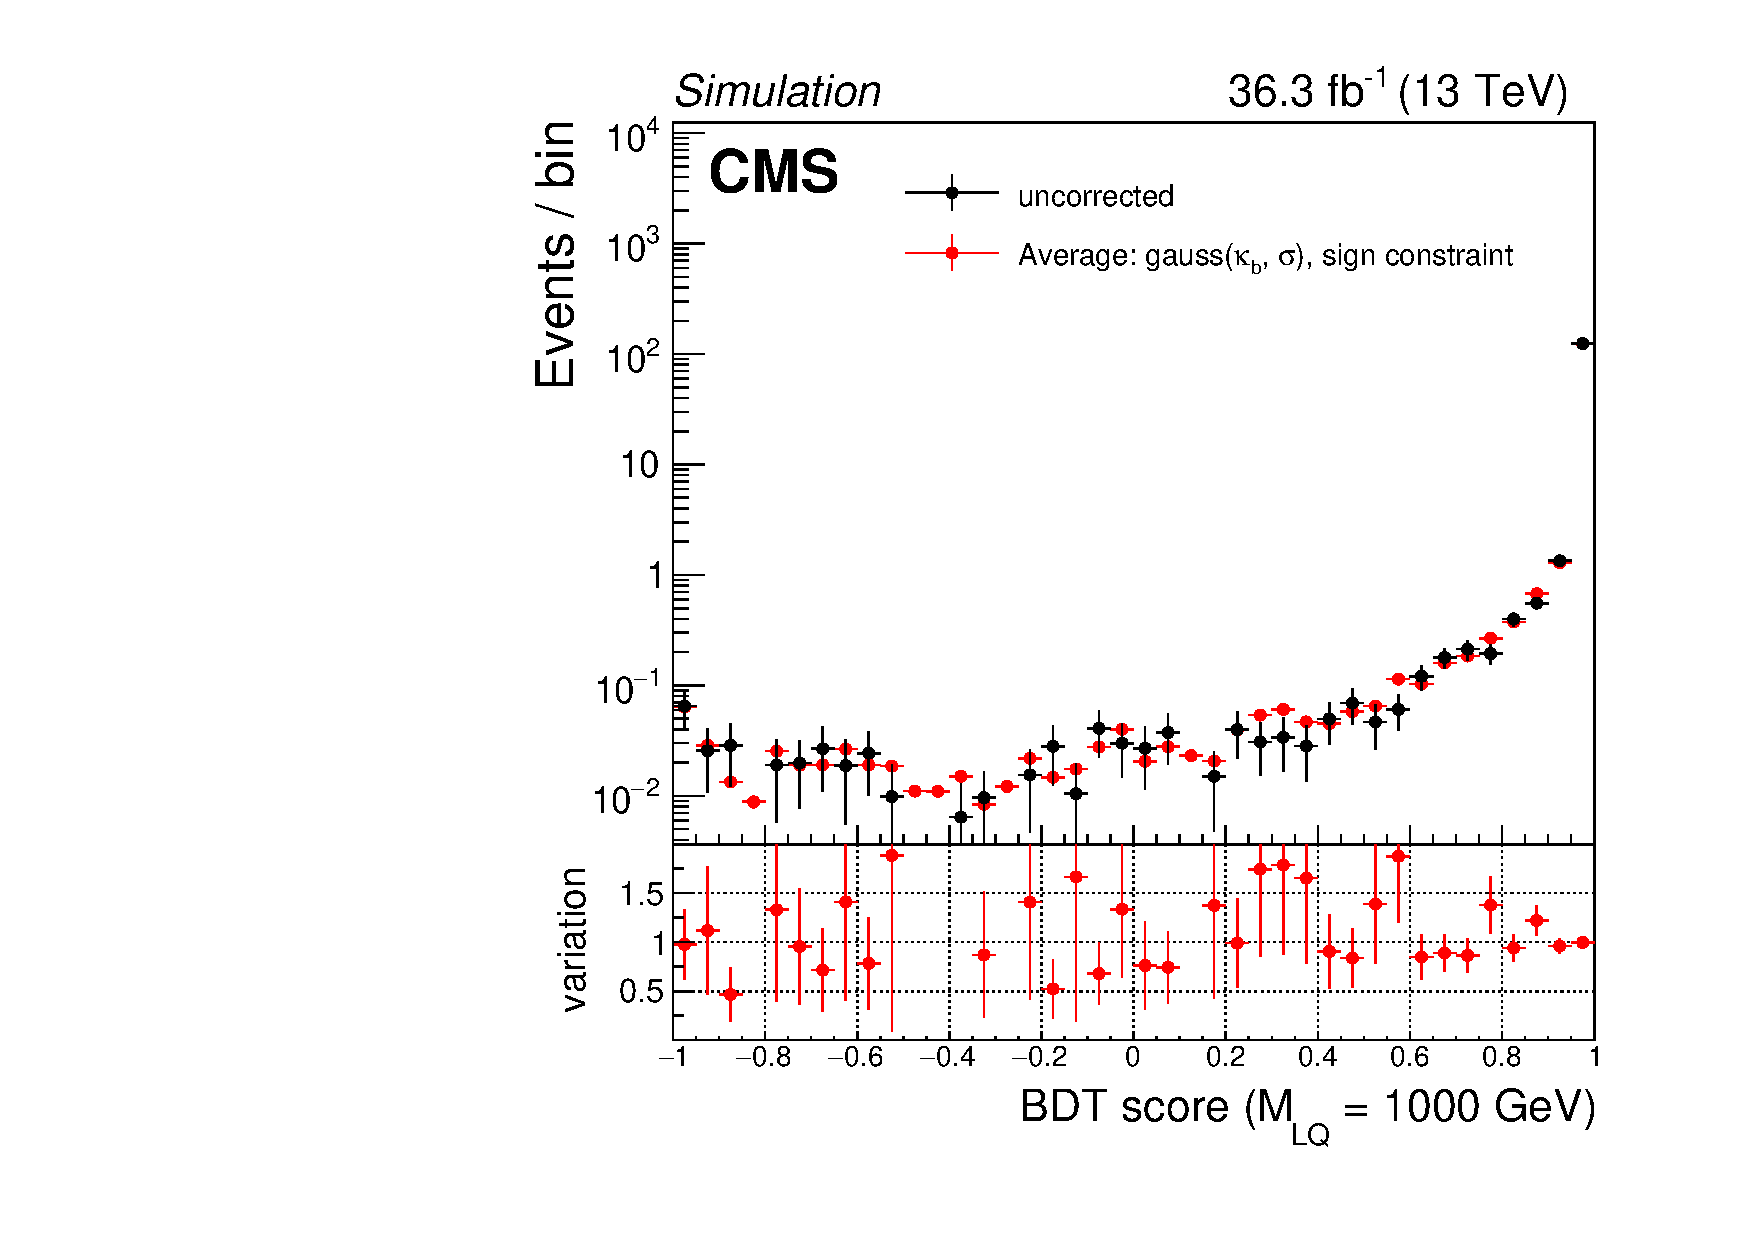
\includegraphics[width=.49\textwidth]{Images/Analysis/GEScaleSystStudy/StudyPlots_2016/SignalM1000/Averages/preSel/GEScaleSystStudyPlot_2016_SignalM1000_Average_preSel_LQToBMu_pair_uubj_BDT_discrim_M1000.pdf}}
    {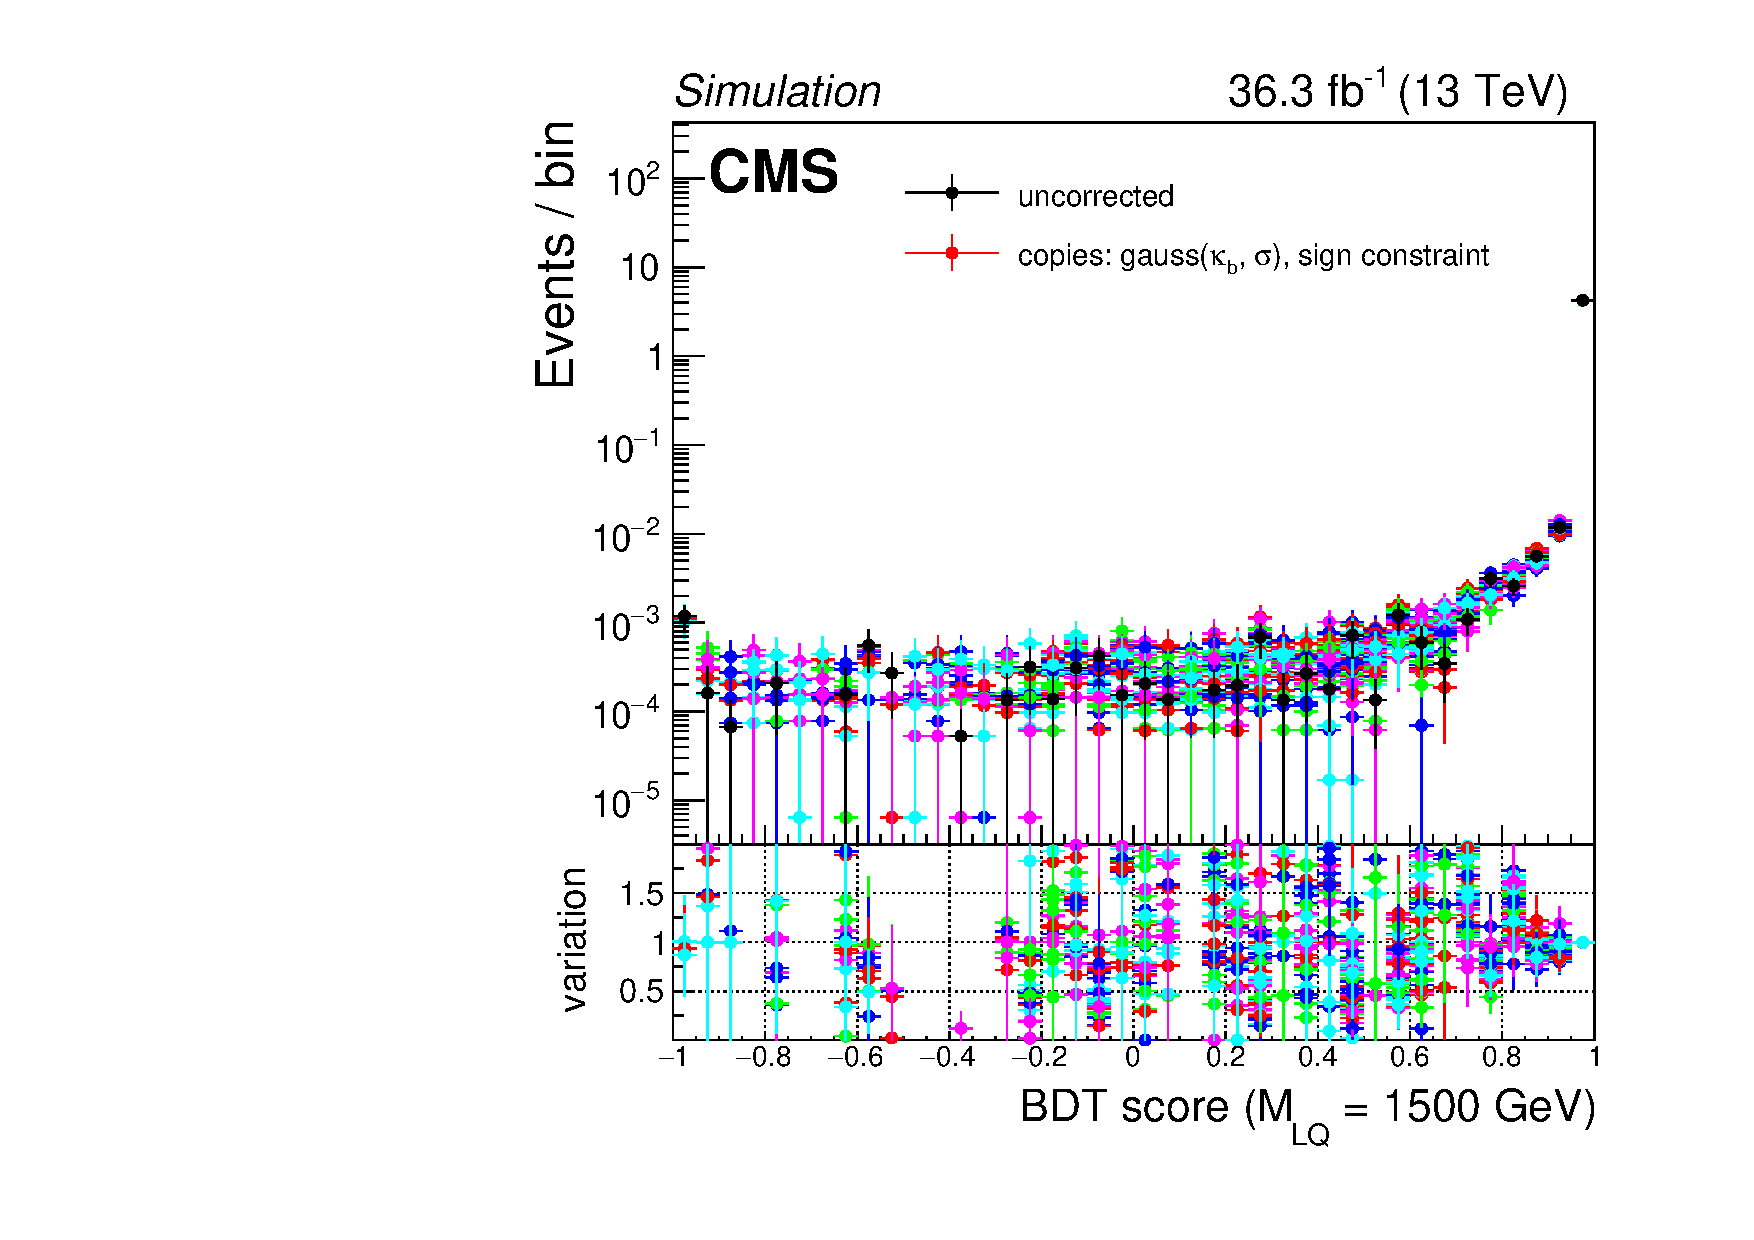
\includegraphics[width=.49\textwidth]{Images/Analysis/GEScaleSystStudy/StudyPlots_2016/SignalM1500/Copies/preSel/GEScaleSystStudyPlot_2016_SignalM1500_Copies_preSel_LQToBMu_pair_uubj_BDT_discrim_M1500.pdf}}
    {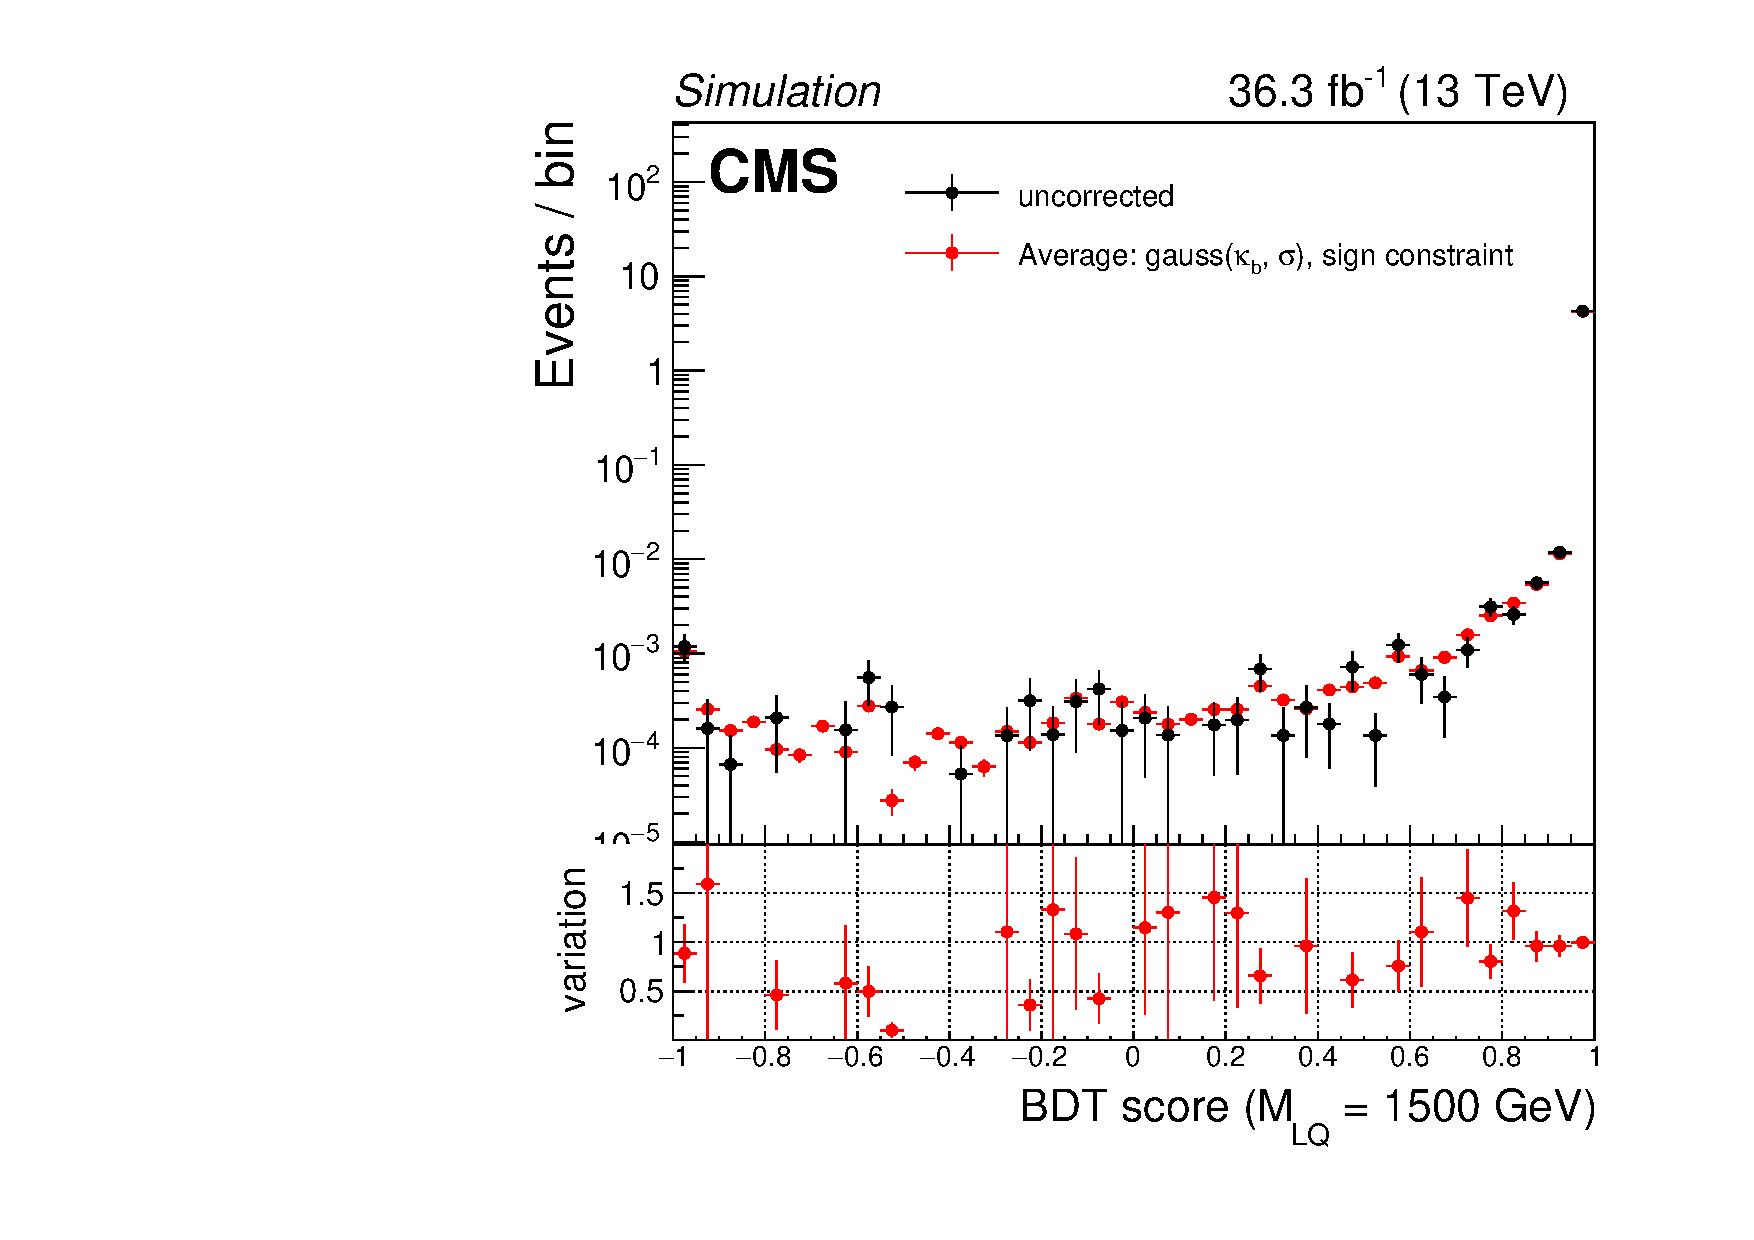
\includegraphics[width=.49\textwidth]{Images/Analysis/GEScaleSystStudy/StudyPlots_2016/SignalM1500/Averages/preSel/GEScaleSystStudyPlot_2016_SignalM1500_Average_preSel_LQToBMu_pair_uubj_BDT_discrim_M1500.pdf}}
    \caption{Left: A comparison between the nominal and statistical replicas of \SI{1000}{GeV} (top) and \SI{1500}{GeV} (bottom) BDT scores. Right: A comparison between the nominal and average over the statistical replicas of \SI{1000}{GeV} (top) and \SI{1500}{GeV} (bottom) BDT scores. Distributions show 2016 signal MC at preselection.}
    \label{figapp:gesysBDTscoresSig1}
\end{figure}

\begin{figure}[H]
    \centering
    {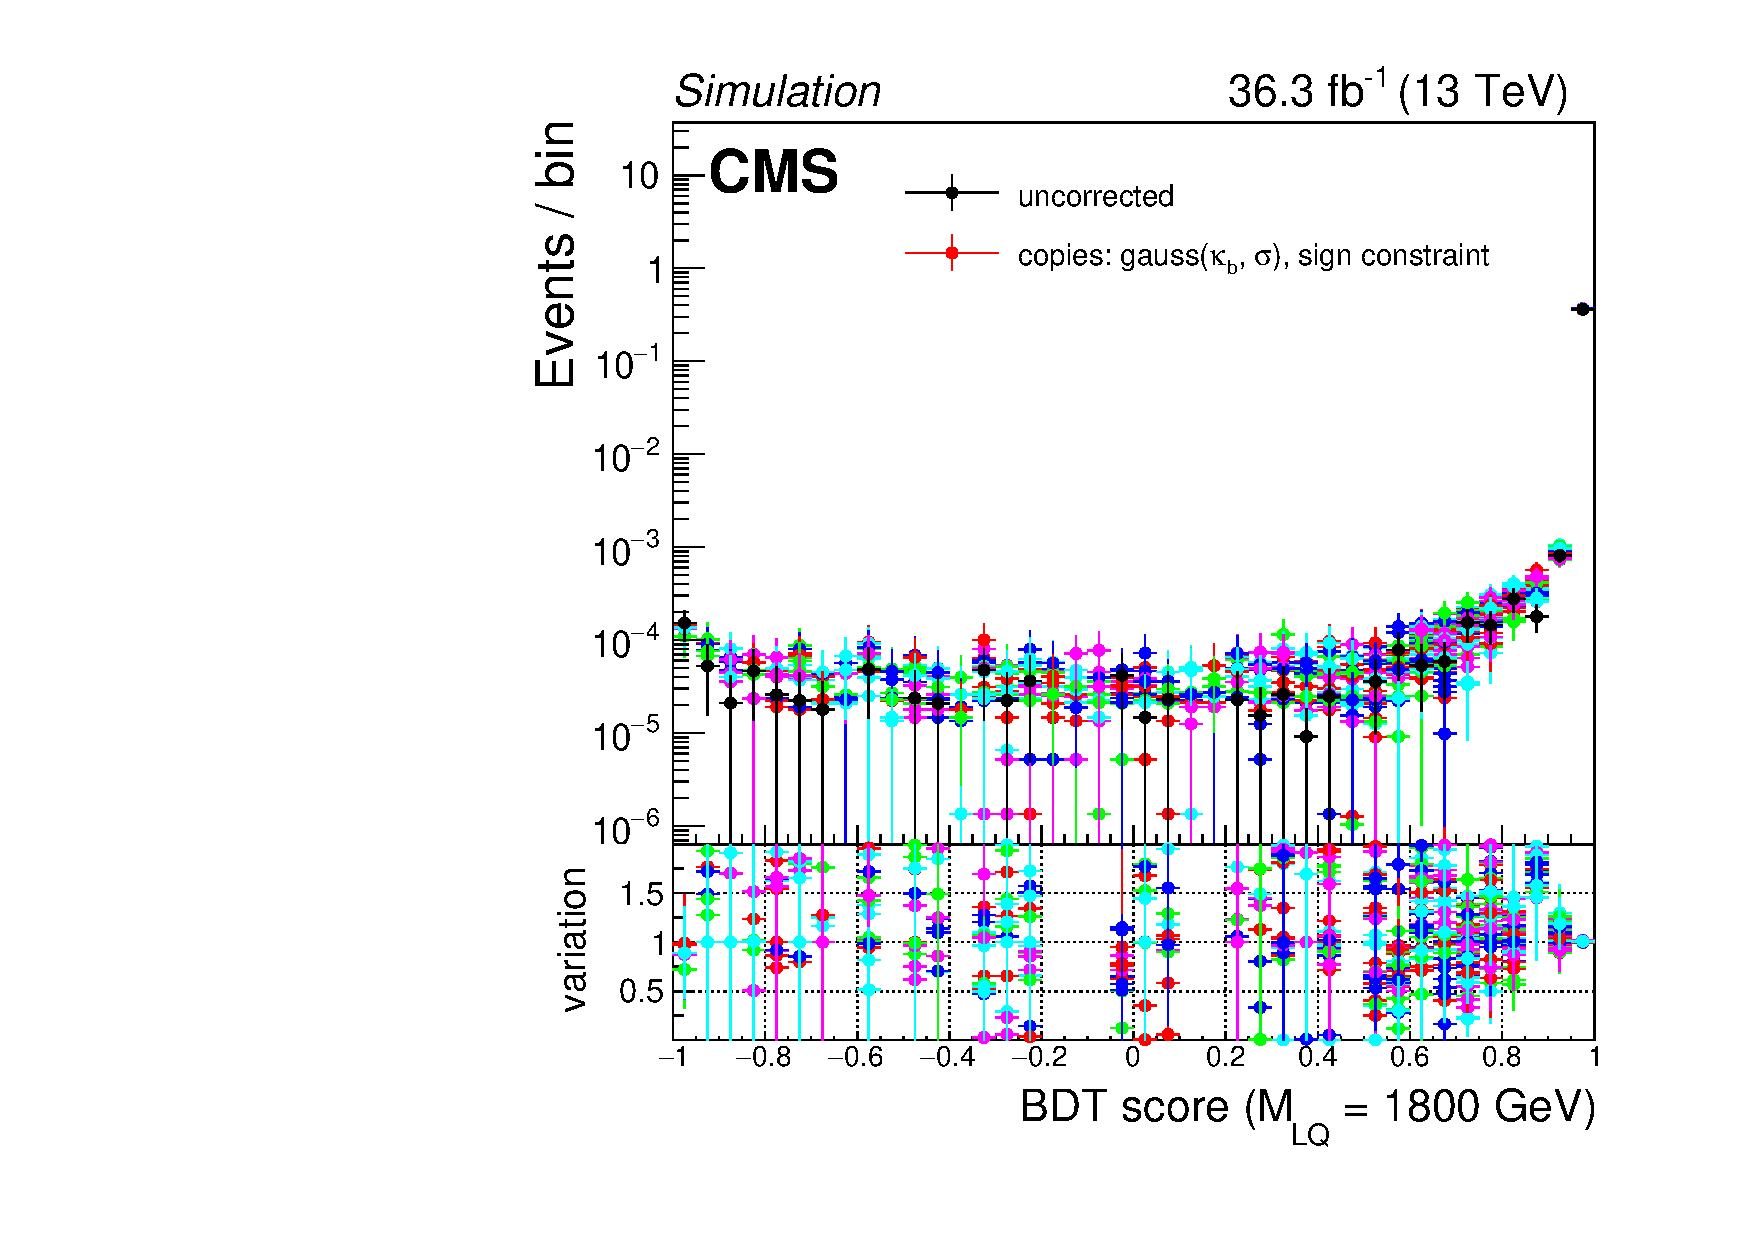
\includegraphics[width=.49\textwidth]{Images/Analysis/GEScaleSystStudy/StudyPlots_2016/SignalM1800/Copies/preSel/GEScaleSystStudyPlot_2016_SignalM1800_Copies_preSel_LQToBMu_pair_uubj_BDT_discrim_M1800.pdf}}
    {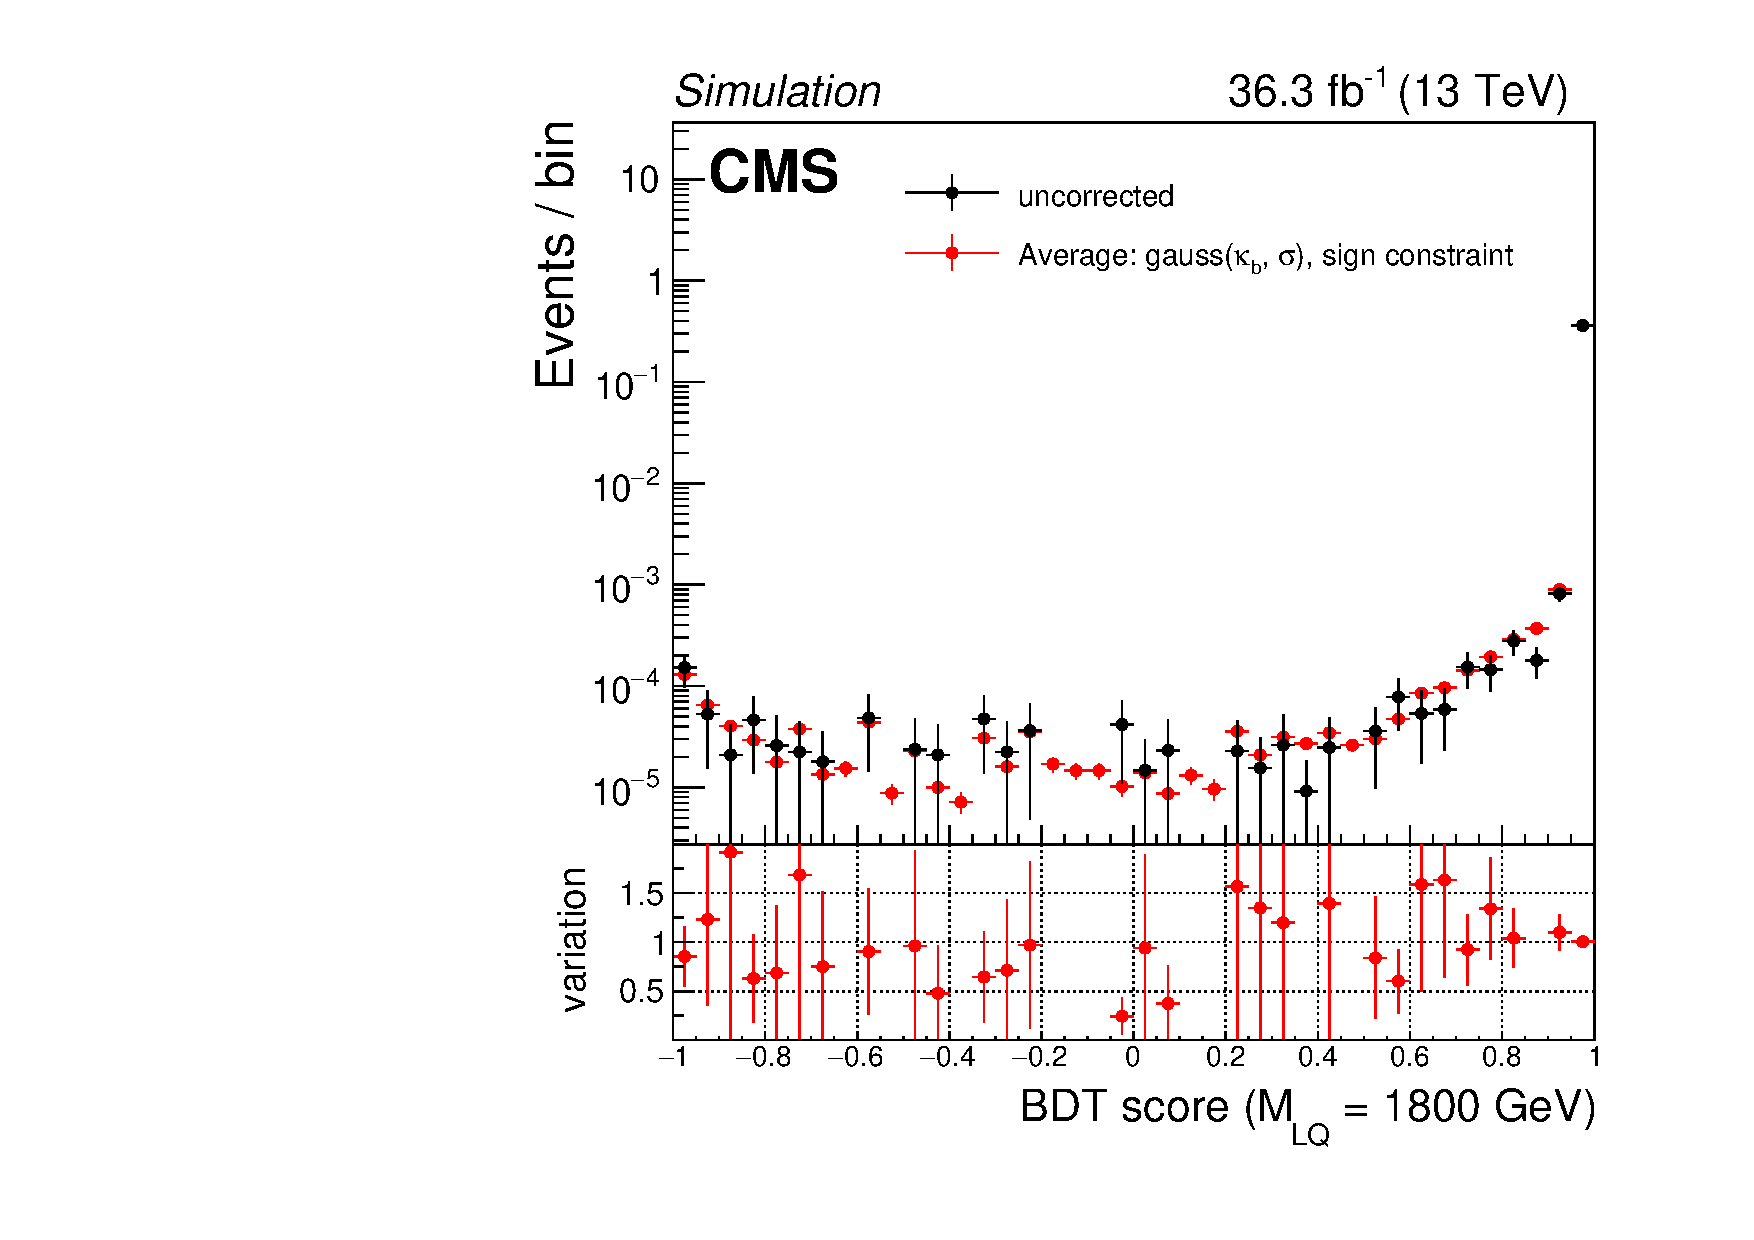
\includegraphics[width=.49\textwidth]{Images/Analysis/GEScaleSystStudy/StudyPlots_2016/SignalM1800/Averages/preSel/GEScaleSystStudyPlot_2016_SignalM1800_Average_preSel_LQToBMu_pair_uubj_BDT_discrim_M1800.pdf}}
    {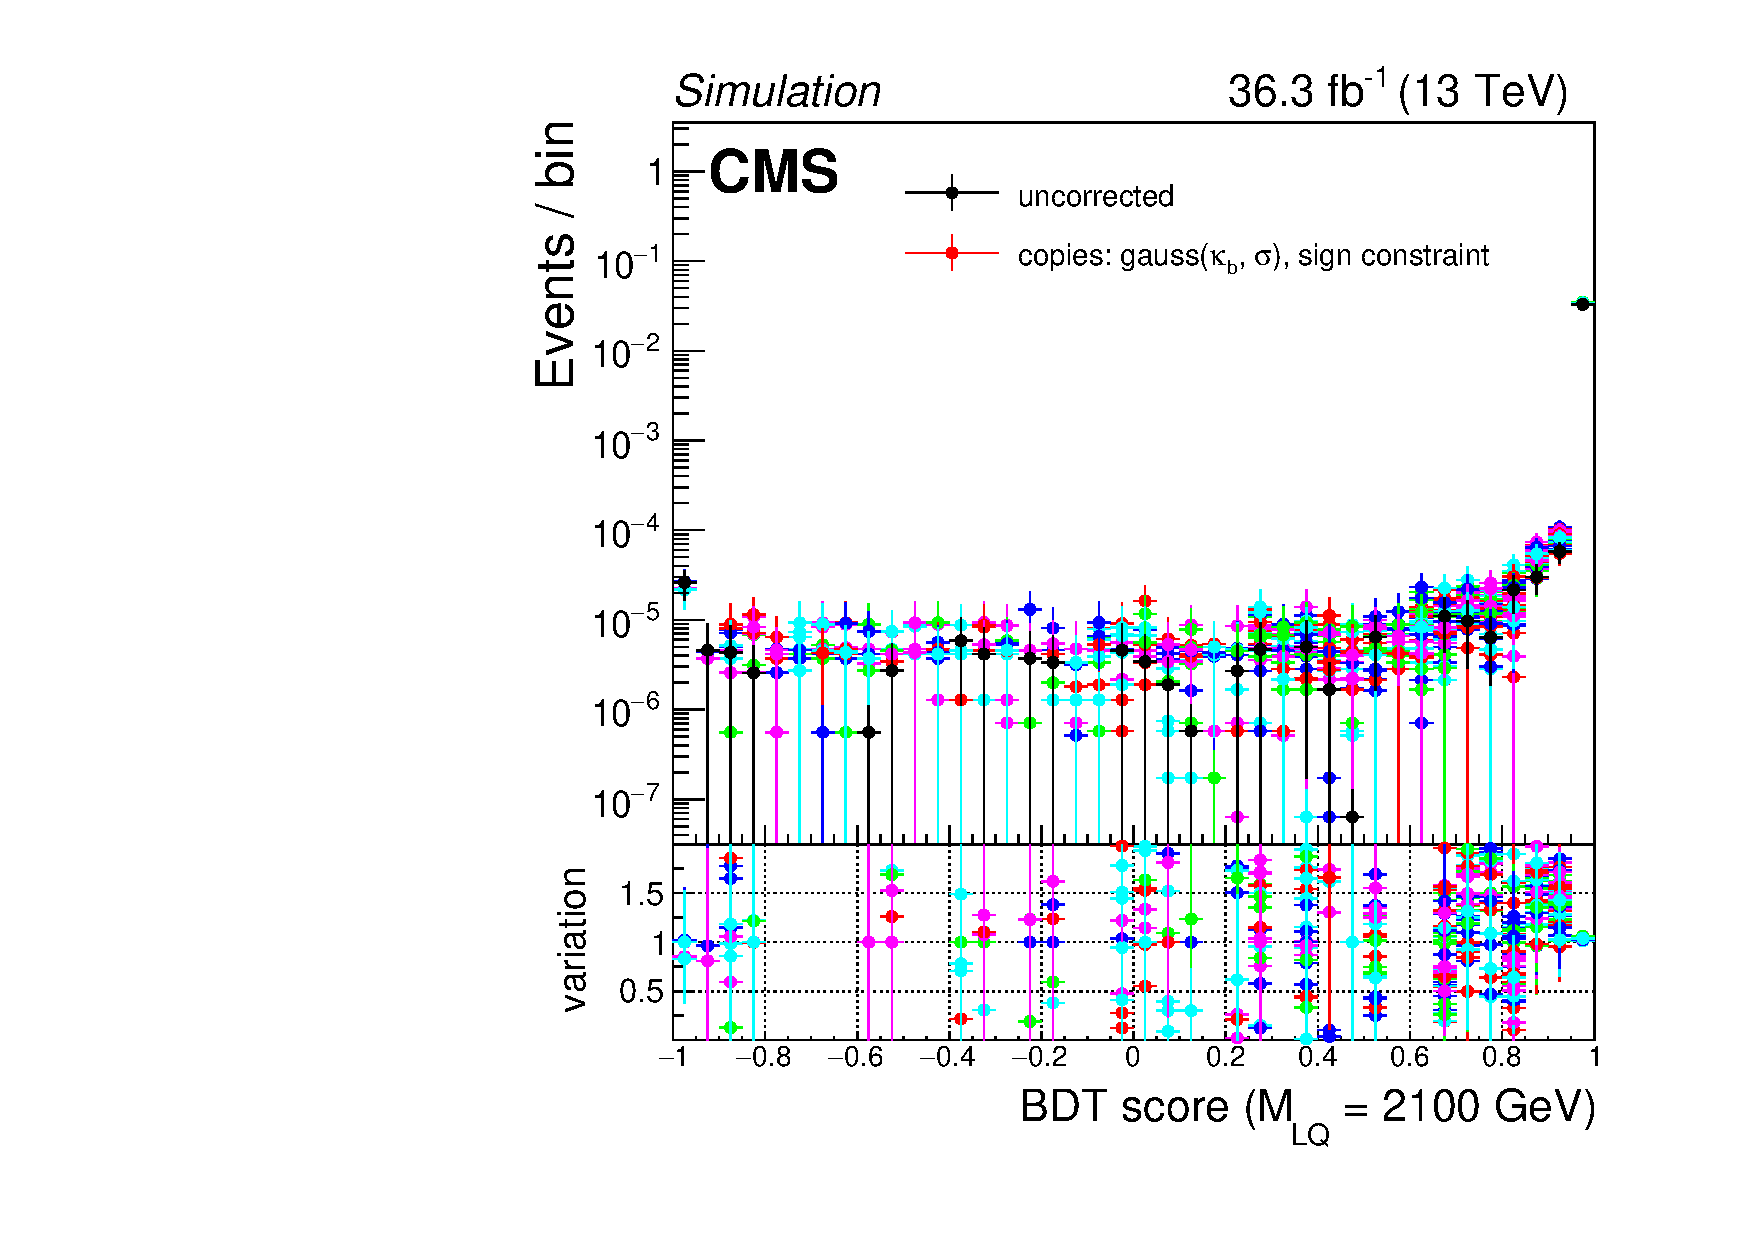
\includegraphics[width=.49\textwidth]{Images/Analysis/GEScaleSystStudy/StudyPlots_2016/SignalM2100/Copies/preSel/GEScaleSystStudyPlot_2016_SignalM2100_Copies_preSel_LQToBMu_pair_uubj_BDT_discrim_M2100.pdf}}
    {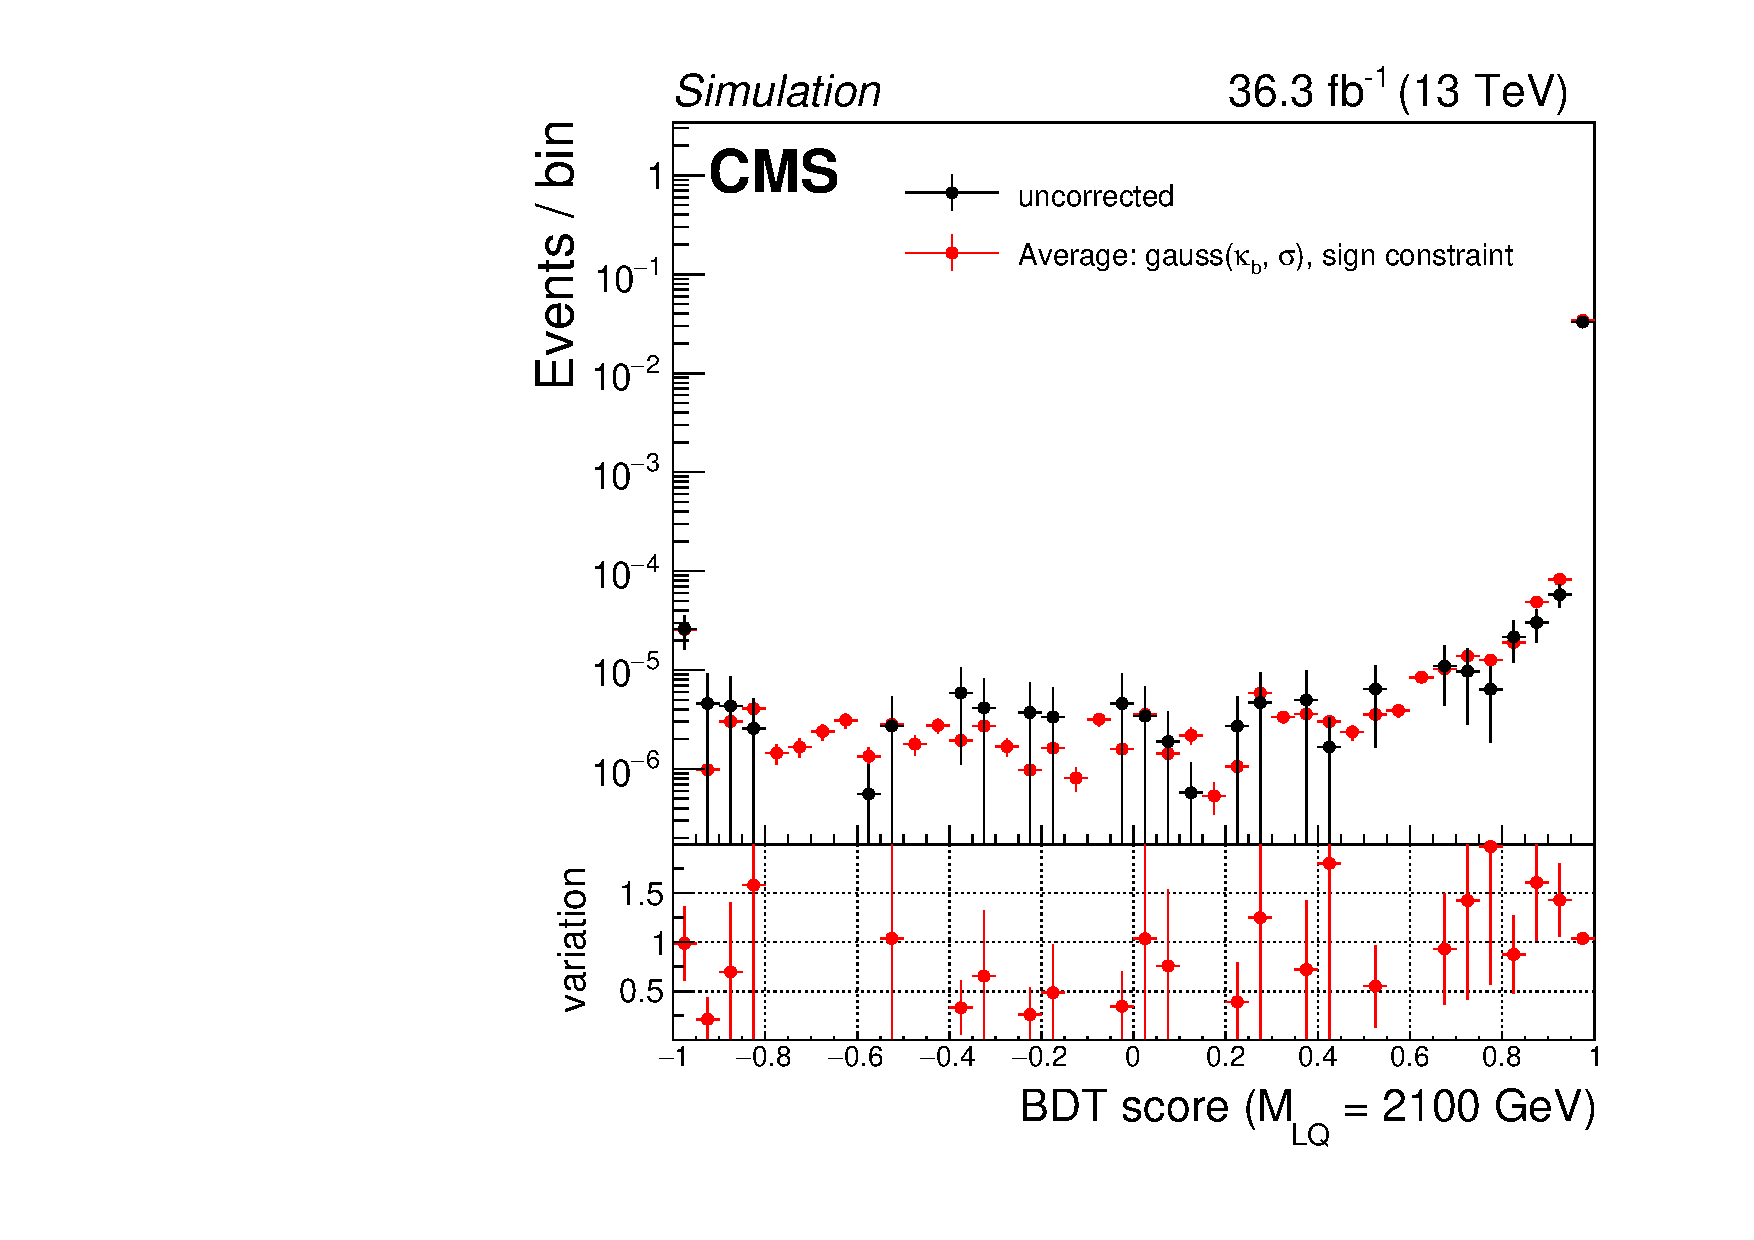
\includegraphics[width=.49\textwidth]{Images/Analysis/GEScaleSystStudy/StudyPlots_2016/SignalM2100/Averages/preSel/GEScaleSystStudyPlot_2016_SignalM2100_Average_preSel_LQToBMu_pair_uubj_BDT_discrim_M2100.pdf}}
    \caption{Left: A comparison between the nominal and statistical replicas of \SI{1800}{GeV} (top) and \SI{2100}{GeV} (bottom) BDT scores. Right: A comparison between the nominal and average over the statistical replicas of \SI{1800}{GeV} (top) and \SI{2100}{GeV} (bottom) BDT scores. Distributions show 2016 signal MC at preselection.}
    \label{figapp:gesysBDTscoresSig2}
\end{figure}

\begin{table}[htbp]
    \begin{center}
        \caption{Muon scale systematic uncertainties estimated with the Generalized Endpoint method and their effect on background in 2016, scanned over several selection working points. All uncertainties are symmetric.}
        \begin{tabular}{lccccc} \hline \hline
            & \multicolumn{5}{c}{Systematic error [\%]} \\
            \LQ Mass [GeV] & enhanced & loose & medium & tight & optimized \\ \hline
            300 & 0.0 & 0.44 & 6.16 & 6.08 & 1.77 \\
            400 & 0.0 & 0.61 & 1.24 & 2.68 & 2.99 \\
            500 & 0.02 & 1.92 & 2.77 & 2.19 & 4.24 \\
            600 & 0.03 & 5.49 & 2.53 & 2.56 & 11.18 \\
            700 & 0.02 & 3.05 & 8.59 & 7.18 & 21.97 \\
            800 & 0.08 & 4.18 & 3.35 & 2.91 & 6.05 \\
            900 & 0.01 & 2.06 & 6.1 & 7.05 & 12.01 \\
            1000 & 0.1 & 5.38 & 3.35 & 22.39 & 13.35 \\
            1100 & 0.18 & 7.54 & 4.01 & 13.23 & 15.09 \\
            1200 & 0.15 & 6.12 & 5.79 & 24.85 & 29.74 \\
            1300 & 0.16 & 12.1 & 22.48 & 9.13 & 48.59 \\
            1400 & 0.49 & 29.06 & 30.76 & 12.21 & 14.11 \\
            1500 & 0.38 & 12.35 & 10.7 & 32.77 & 22.61 \\
            1600 & 1.22 & 21.9 & 31.33 & 45.47 & 7.02 \\
            1700 & 0.07 & 25.01 & 30.2 & 112.19 & 63.08 \\
            1800 & 4.38 & 16.45 & 20.2 & 22.11 & 22.35 \\
            1900 & 3.27 & 36.36 & 12.44 & 17.36 & 25.52 \\
            2100 & 1.78 & 86.8 & 239.12 & 293.8 & 321.2 \\
            2200 & 3.16 & 31.46 & 4.65 & 12.36 & 249.65 \\
            2300 & 1.44 & 97.77 & 112.71 & 234.21 & 588.68 \\
            2400 & 9.75 & 606.19 & 548.16 & 202.56 & 192.41 \\
            2500 & 1.92 & 106.58 & 106.67 & 40.07 & 259.96 \\
            2600 & 0.03 & 7.01 & 7.01 & 7.01 & 7.01 \\
            2700 & 1.98 & 105.55 & 261.41 & 177.83 & 177.83 \\
            2800 & 0.43 & 68.36 & 38.91 & 26.41 & 12.74 \\
            2900 & 3.28 & 626.01 & 487.37 & 54.57 & 140.7 \\
            3000 & 0.95 & 92.55 & 52.33 & 197.05 & 197.05 \\
            3500 & 46.79 & 206.29 & 213.06 & 195.41 & 212.36 \\
            4000 & 60.05 & 5.16 & 33.58 & 135.41 & 112.51 \\ \hline\hline
        \end{tabular}
        \label{tab:gesystbkg}
    \end{center}
\end{table}

\begin{table}[htbp]
    \begin{center}
        \caption{Muon scale systematic uncertainties estimated with the Generalized Endpoint method and their effect on signal in 2016, scanned over several selection working points. All uncertainties are ymmetric.}
        \begin{tabular}{lccccc} \hline \hline
            & \multicolumn{5}{c}{Systematic error [\%]} \\
            \LQ Mass [GeV] & enhanced & loose & medium & tight & optimized \\ \hline
            300 & 0.02 & 0.1 & 0.09 & 0.33 & 0.65 \\
            400 & 0.0 & 0.0 & 0.02 & 0.26 & 0.28 \\
            500 & 0.02 & 0.04 & 0.03 & 0.13 & 0.48 \\
            600 & 0.0 & 0.03 & 0.04 & 0.08 & 0.2 \\
            700 & 0.01 & 0.02 & 0.04 & 0.09 & 0.39 \\
            800 & 0.02 & 0.04 & 0.06 & 0.03 & 0.16 \\
            900 & 0.05 & 0.08 & 0.08 & 0.1 & 0.11 \\
            1000 & 0.11 & 0.12 & 0.18 & 0.33 & 0.51 \\
            1100 & 0.05 & 0.06 & 0.08 & 0.08 & 0.14 \\
            1200 & 0.13 & 0.14 & 0.15 & 0.16 & 0.2 \\
            1300 & 0.12 & 0.12 & 0.14 & 0.13 & 0.18 \\
            1400 & 0.16 & 0.16 & 0.17 & 0.21 & 0.21 \\
            1500 & 0.18 & 0.18 & 0.18 & 0.21 & 0.21 \\
            1600 & 0.15 & 0.16 & 0.15 & 0.18 & 0.18 \\
            1700 & 0.11 & 0.12 & 0.1 & 0.14 & 0.14 \\
            1800 & 0.15 & 0.14 & 0.14 & 0.18 & 0.18 \\
            1900 & 0.09 & 0.1 & 0.1 & 0.11 & 0.11 \\
            2100 & 0.03 & 0.03 & 0.02 & 0.0 & 0.0 \\
            2200 & 0.09 & 0.09 & 0.09 & 0.08 & 0.06 \\
            2300 & 0.1 & 0.1 & 0.11 & 0.09 & 0.11 \\
            2400 & 0.18 & 0.18 & 0.19 & 0.18 & 0.18 \\
            2500 & 0.23 & 0.24 & 0.24 & 0.24 & 0.22 \\
            2600 & 0.27 & 0.28 & 0.28 & 0.28 & 0.28 \\
            2700 & 0.27 & 0.27 & 0.27 & 0.25 & 0.25 \\
            2800 & 0.38 & 0.38 & 0.37 & 0.37 & 0.35 \\
            2900 & 0.3 & 0.32 & 0.32 & 0.31 & 0.28 \\
            3000 & 0.41 & 0.41 & 0.42 & 0.41 & 0.41 \\
            3500 & 0.4 & 0.4 & 0.4 & 0.39 & 0.4 \\
            4000 & 0.48 & 0.48 & 0.48 & 0.47 & 0.47 \\ \hline\hline
        \end{tabular}
        \label{tab:gesystsig}
    \end{center}
\end{table}